\documentclass[11pt]{article}

\usepackage{a4wide}
\usepackage[utf8]{inputenc}
\usepackage[russian]{babel}
\usepackage{graphicx}
\usepackage{amsmath}
\usepackage{float}
\usepackage{hyperref}

\DeclareMathOperator{\sinc}{sinc}
\DeclareMathOperator{\arctg}{arctg}

\begin{document}

\thispagestyle{empty}

\begin{center}
\ \vspace{-3cm}

\includegraphics[width=0.5\textwidth]{msu.eps}\\
{\scshape Московский государственный университет имени М.~В.~Ломоносова}\\
Факультет вычислительной математики и кибернетики\\
Кафедра системного анализа

\vfill

{\LARGE Отчет по практикуму}

\vspace{1cm}

{\Huge\bfseries <<Применение быстрого преобразования Фурье в Matlab>>}
\end{center}

\vspace{1cm}

\begin{flushright}
  \large
  \textit{Студент 315 группы}\\
  М.\,В.~Миловидов

  \vspace{5mm}

  \textit{Руководитель практикума}\\
  к.ф.-м.н., доцент П.\,А.~Точилин
\end{flushright}

\vfill

\begin{center}
Москва, 2024
\end{center}

\newpage
\section{Постановка задачи}

Получить аппроксимацию преобразования Фурье F($\lambda$) для каждой функции f(t) из следующего набора:
\newline
\begin{equation} \arctg(t/2) - \arctg(t), \end{equation}

\begin{equation}
\begin{cases}
\sin(2t), 3|t| \leq 1,\\
0, \text{иначе}.
\end{cases},
\end{equation}

\begin{equation} \frac{e^{-2|t|}}{1+2\arctg^2(t)}, \end{equation}

\begin{equation} \frac{\sin(t^3)}{t^2}, \end{equation}

при помощи быстрого преобразования Фурье (БПФ), выбирая различные шаги дискретизации
исходной функции и различные окна, ограничивающие область определения f(t). Построить графики F($\lambda$). Для
первых двух функций f(t) вычислить F($\lambda$) в явном виде и сравнить графики F($\lambda$), полученные из аналитического
представления F($\lambda$) и из аппроксимации через БПФ.
\newline

Должна быть реализована функция plotFT(hFigure, fHandle, fFTHandle, step, inpLimVec, outLimVec).
Входные аргументы этой функции следующие:
\newline

hFigure — handle существующей фигуры c 2 осями для графиков, в которую осуществляется вывод графиков. При от-
сутствии осей (пустая фигура) должны быть созданы отдельные оси для вывода соответственно действительной
и мнимой части преобразования Фурье F($\lambda$). При наличии осей выводить новые графики в них, предварительно
очистив их от старых графиков (о том, как это сделать, см. комментарии ниже о хранении метаинформации в
свойстве UserData). При этом при отсутствии необязательного параметра outLimVec (см. ниже) пределы осей
абсцисс не должны меняться (и быть одинаковыми для вещественной и мнимой части F($\lambda)$).
\newline

fHandle — function handle для функции f(t) (для f(t) из набора, указанного на стр. 8 данного файла, соответствующие
функции должны быть также реализованы под именами func1(t), func2(t), func3(t) и func4(t), так что в
fHandle можно передавать @func1, @func2, @func3 и @func4, соответственно).
\newline

fFTHandle — либо function handle, либо пустой массив []. В случае function handle содержит handle функции, задаю-
щей аналитически вычисленное преобразование Фурье F($\lambda$) для первых двух функций f(t) из набора, указанного
на стр. 8 данного файла (точное преобразование Фурье в этом случае должно выводиться вместе с приближен-
ным). Соответствующие преобразования должны быть реализованы под именами ftfunc1(l), ftfunc2(l), так
что в fFTHandle можно передавать @ftfunc1, @ftfunc2, соответственно. Если fFTHandle содержит пустой массив
[], на осях выводятся только численные аппроксимации преобразования Фурье.
step — положительное число, задающее шаг дискретизации $\Delta$ t.
\newline

inpLimVec — вектор-строка из двух элементов, задающий окно [a, b] для f(t) (первый элемент вектора содержит a,
второй — b, a < b, причем не обязательно a = −b).
\newline

outLimVec — вектор-строка из двух элементов, задающий окно для вывода преобразования Фурье [c, d] (первый эле-
мент вектора содержит c, второй — d, c < d). То есть при выводе пределы оси для λ должны задаваться
пользователем через этот параметр (таким образом, может выводиться только часть графика преобразования
Фурье). Этот параметр может быть опциональным (то есть не передаваться в функцию). В таком случае окно
для вывода берется из пределов осей абсцисс (при наличии на фигуре уже существующих правильных осей).
Если же старых осей нет, то это окно может как-то разумно выбираться.
Замечание. При выводе преобразования Фурье в окне [c, d] должны быть подсчитаны только те значения
спектра, которые попадают в это окно. То есть не допускается расчёт спектра на очень большом интервале (”с
запасом”), а далее вывод небольшой его части.



\section{Вычисление fft}

В начале алгоритма считается число точек разбиения N и пересчитывается шаг step, чтобы интервал ровно делился на N. Далее считается сетка разбиения сигнала, шаг спектра lstep = 2 * pi / T, где T - период разбиения. Далее по окну спектра считаются граничные точки nA и nB, попадающие в это окно, и разбиение спектра l = 0:lstep:(N-1)*lstep. Считается быстрое преобразование Фурье при помощи функции fft, оно домножается на шаг step для получения нужного маштаба спектра, а также на вектор экспонент exp(-1i * a * l) для сдвига a в 0. Получившийся вектор дублируется для заполнения всего нужного промежутка.

\section{Вычисление преобразования Фурье для функций 1 и 2}
\[ f_1(t) = \arctg(t/2) - \arctg(t).\]
\[F(\lambda) = \int_{-\infty}^{+\infty} (\arctg(t/2) - \arctg(t))e^{-i\lambda t} dt = \{\lambda \neq 0\} = -\frac{1}{i\lambda}(\arctg(t/2) - \arctg(t))e^{-i\lambda t}\Big|_{-\infty}^{+\infty} +\] 
\[+ \frac{1}{i\lambda}\int_{-\infty}^{+\infty} \left( \frac{1}{1 + \frac{t^2}{4}} \cdot\frac{1}{2} - \frac{1}{1 + t^2} \right) e^{-i\lambda t}dt = \frac{1}{i\lambda}\int_{-\infty}^{+\infty} \left( \frac{2}{t^2 + 4} - \frac{1}{t^2 + 1} \right) e^{-i\lambda t}dt = \]
Посчитаем интеграл по лемме Жордана. У каждой дроби две особые точки $\pm 2i$ и $\pm i$, из них в верхней полуплоскости находится +i и +2i. Они является полюсами первого порядка, в итоге имеем
\[ = \frac{2\pi i}{i \lambda} \left( \lim\limits_{t \to 2i} \frac{2}{t^2 + 4}e^{i\lambda t}(t - 2i) - \lim\limits_{t \to i} \frac{1}{t^2 + 1}e^{i\lambda t}(t - i) \right) = \frac{2\pi}{\lambda} \left( \lim\limits_{t \to 2i} \frac{2}{t + 2i}e^{i\lambda t} - \lim\limits_{t \to i} \frac{1}{t + i}e^{i\lambda t} \right) = \]
\[ = \frac{2\pi}{\lambda} \left( \frac{1}{2i}e^{-2\lambda} - \frac{1}{2i}e^{-\lambda} \right) = \frac{i\pi}{\lambda}(e^{-\lambda} - e^{-2\lambda}).\]
Случай $\lambda = 0$:
\[\int_{-\infty}^{+\infty} (\arctg(t/2) - \arctg(t)) dt = 0.\]
\newline
\begin{equation}
f_2(t) = 
\begin{cases}
\sin(2t), 3|t| \leq 1,\\
0, \text{иначе}.
\end{cases}
\end{equation}
\newline
1) $\lambda \neq \pm 2:$
\[F(\lambda) = \int_{-\frac{1}{3}}^{+\frac{1}{3}}\sin(2t)e^{-i\lambda t} dt = i\int_{-\frac{1}{3}}^{+\frac{1}{3}}\sin(2t)\sin(\lambda t) dt = \frac{i}{2}\int_{-\frac{1}{3}}^{+\frac{1}{3}} \left( \cos(2- \lambda) - \cos(2 + \lambda))\sin(\lambda t \right) dt =\]
\[= \frac{i}{2} \left( \frac{1}{2 - \lambda}\sin(2 - \lambda)t\Big|_{-\frac{1}{3}}^{+\frac{1}{3}} - \frac{1}{2 + \lambda}\sin(2 + \lambda)t\Big|_{-\frac{1}{3}}^{+\frac{1}{3}} \right) = i \left( \frac{\sin\frac{2 - \lambda}{3}}{2 - \lambda} - \frac{\sin\frac{2 + \lambda}{3}}{2 + \lambda} \right) = \frac{i}{3} \left( \sinc\frac{2-\lambda}{3 \pi} - \sinc\frac{2+\lambda}{3 \pi} \right). \]
\newline
2) $\lambda = \pm 2:$
\[F(\lambda) = \pm i\int_{-\frac{1}{3}}^{+\frac{1}{3}}\sin^2(2t) dt = \pm \frac{i}{2}\int_{-\frac{1}{3}}^{+\frac{1}{3}}(1 - \cos4t) dt = \pm \frac{i}{2} \left( \frac{2}{3} - \frac{\sin4t}{4}\Big|_{-\frac{1}{3}}^{+\frac{1}{3}} \right) = \pm \frac{i}{2} \left( \frac{2}{3} - \frac{2\sin\frac{4}{3}}{4} \right) =\]
\[= \pm\frac{i}{3} \left( 1 - \sinc\frac{4}{3 \pi} \right) = \frac{i}{3} \left( \sinc\frac{2-\lambda}{3 \pi} - \sinc\frac{2+\lambda}{3 \pi} \right).\]
\[F(\lambda) = \frac{i}{3} \left( \sinc\frac{2-\lambda}{3 \pi} - \sinc\frac{2+\lambda}{3 \pi} \right) \ \forall \lambda.\]
\section{Полученные графики}


\newline
\[f(t) = \arctg(t/2) - \arctg(t),\ F(\lambda) = \begin{cases}\frac{i\pi}{\lambda}(e^{-\lambda} - e^{-2\lambda}), \lambda \neq 0 \\ 0, \lambda = 0\end{cases}.\]
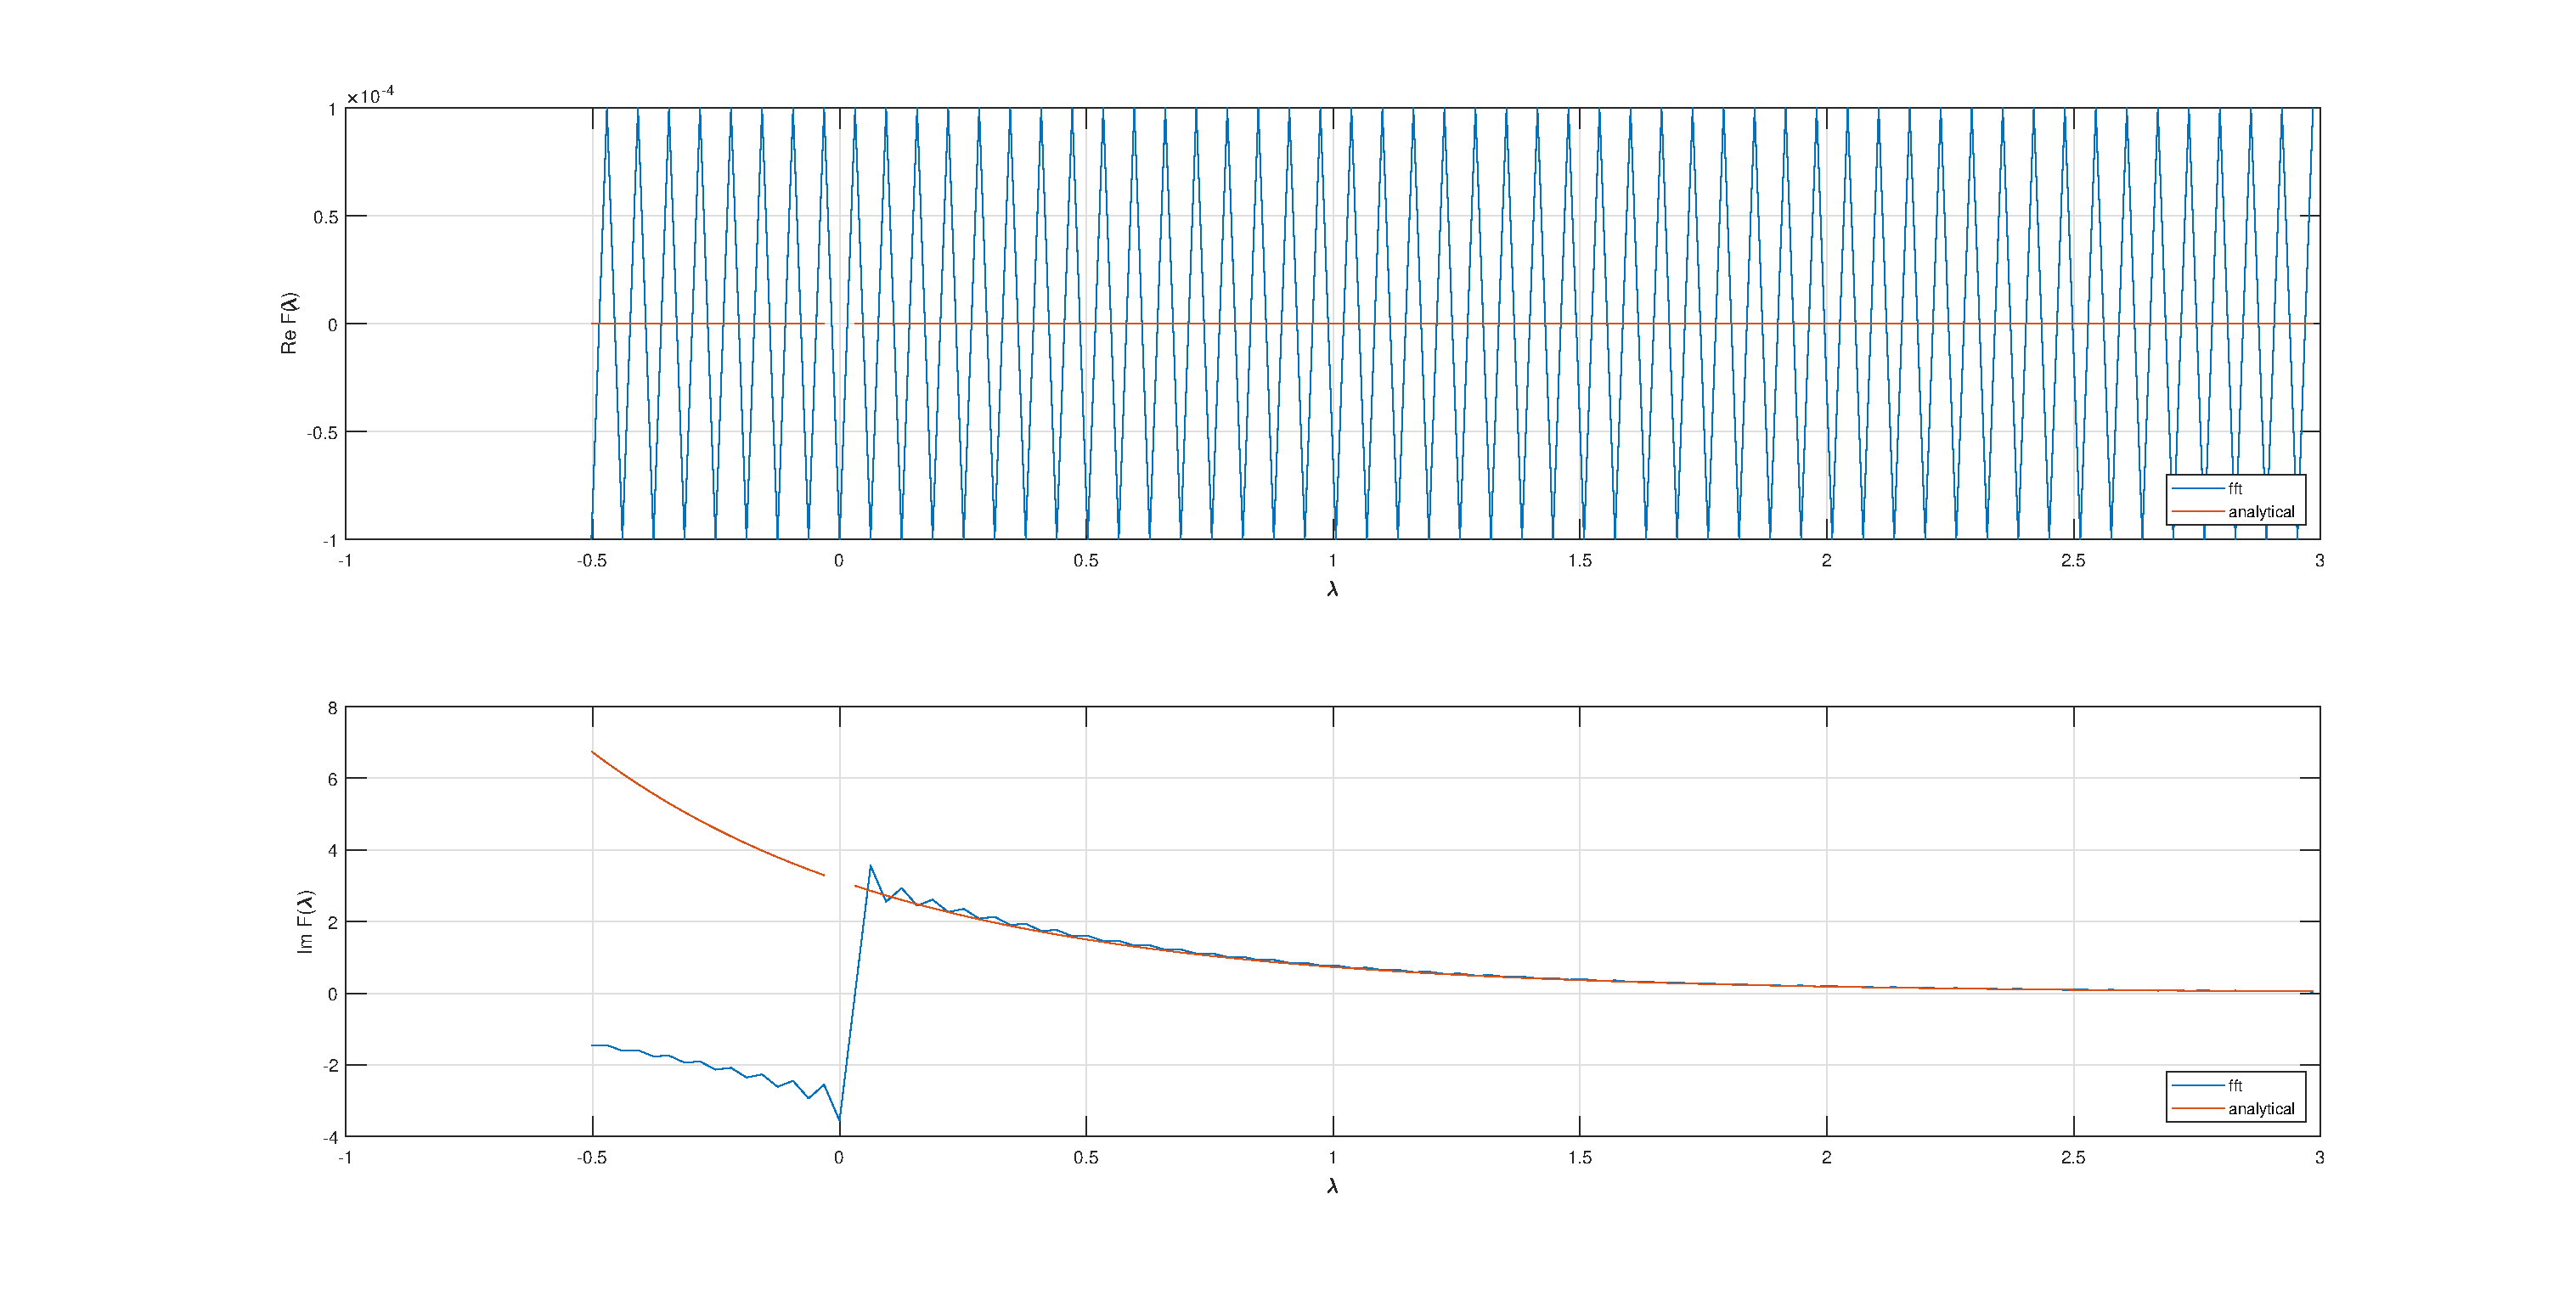
\includegraphics[width=1\textwidth]{f1.eps}

\[ f(t) = \begin{cases} \sin(2t), 3|t| \leq 1\\ 0, \text{иначе} \end{cases},\ F(\lambda) = \frac{i}{3} \left( \sinc\frac{2-\lambda}{3 \pi} - \sinc\frac{2+\lambda}{3 \pi} \right).\]
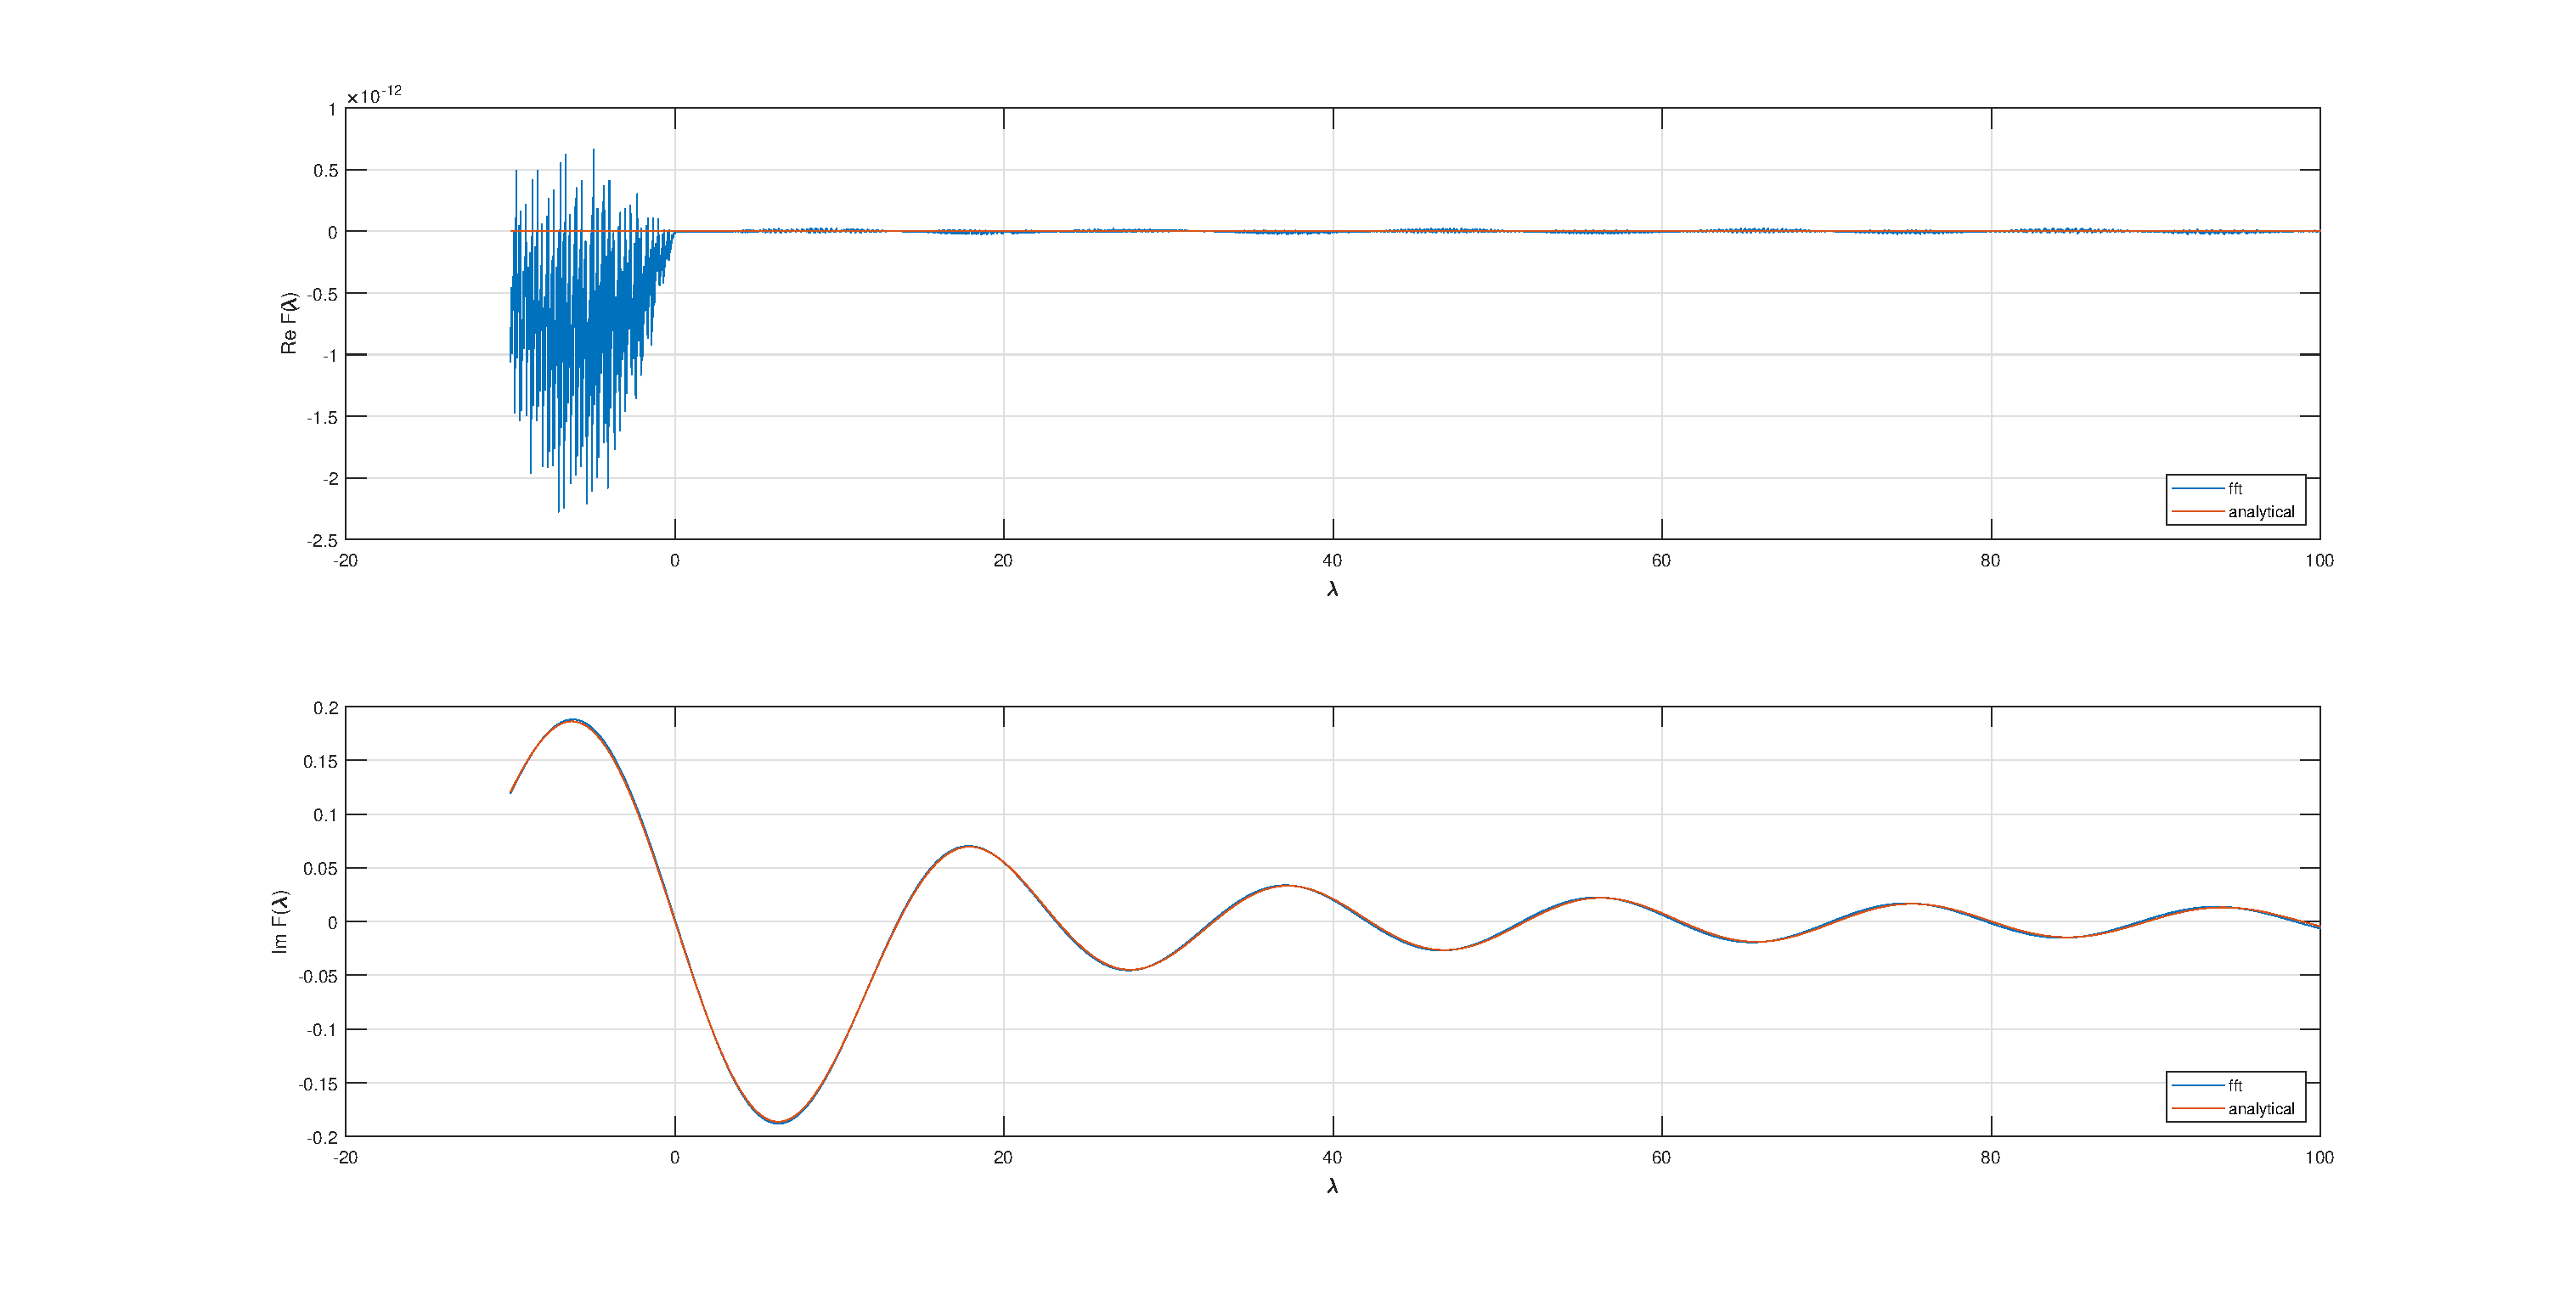
\includegraphics[width=1\textwidth]{f2.eps}
\[f(t) = \frac{e^{-2|t|}}{1+2\arctg^2(t)}.\]
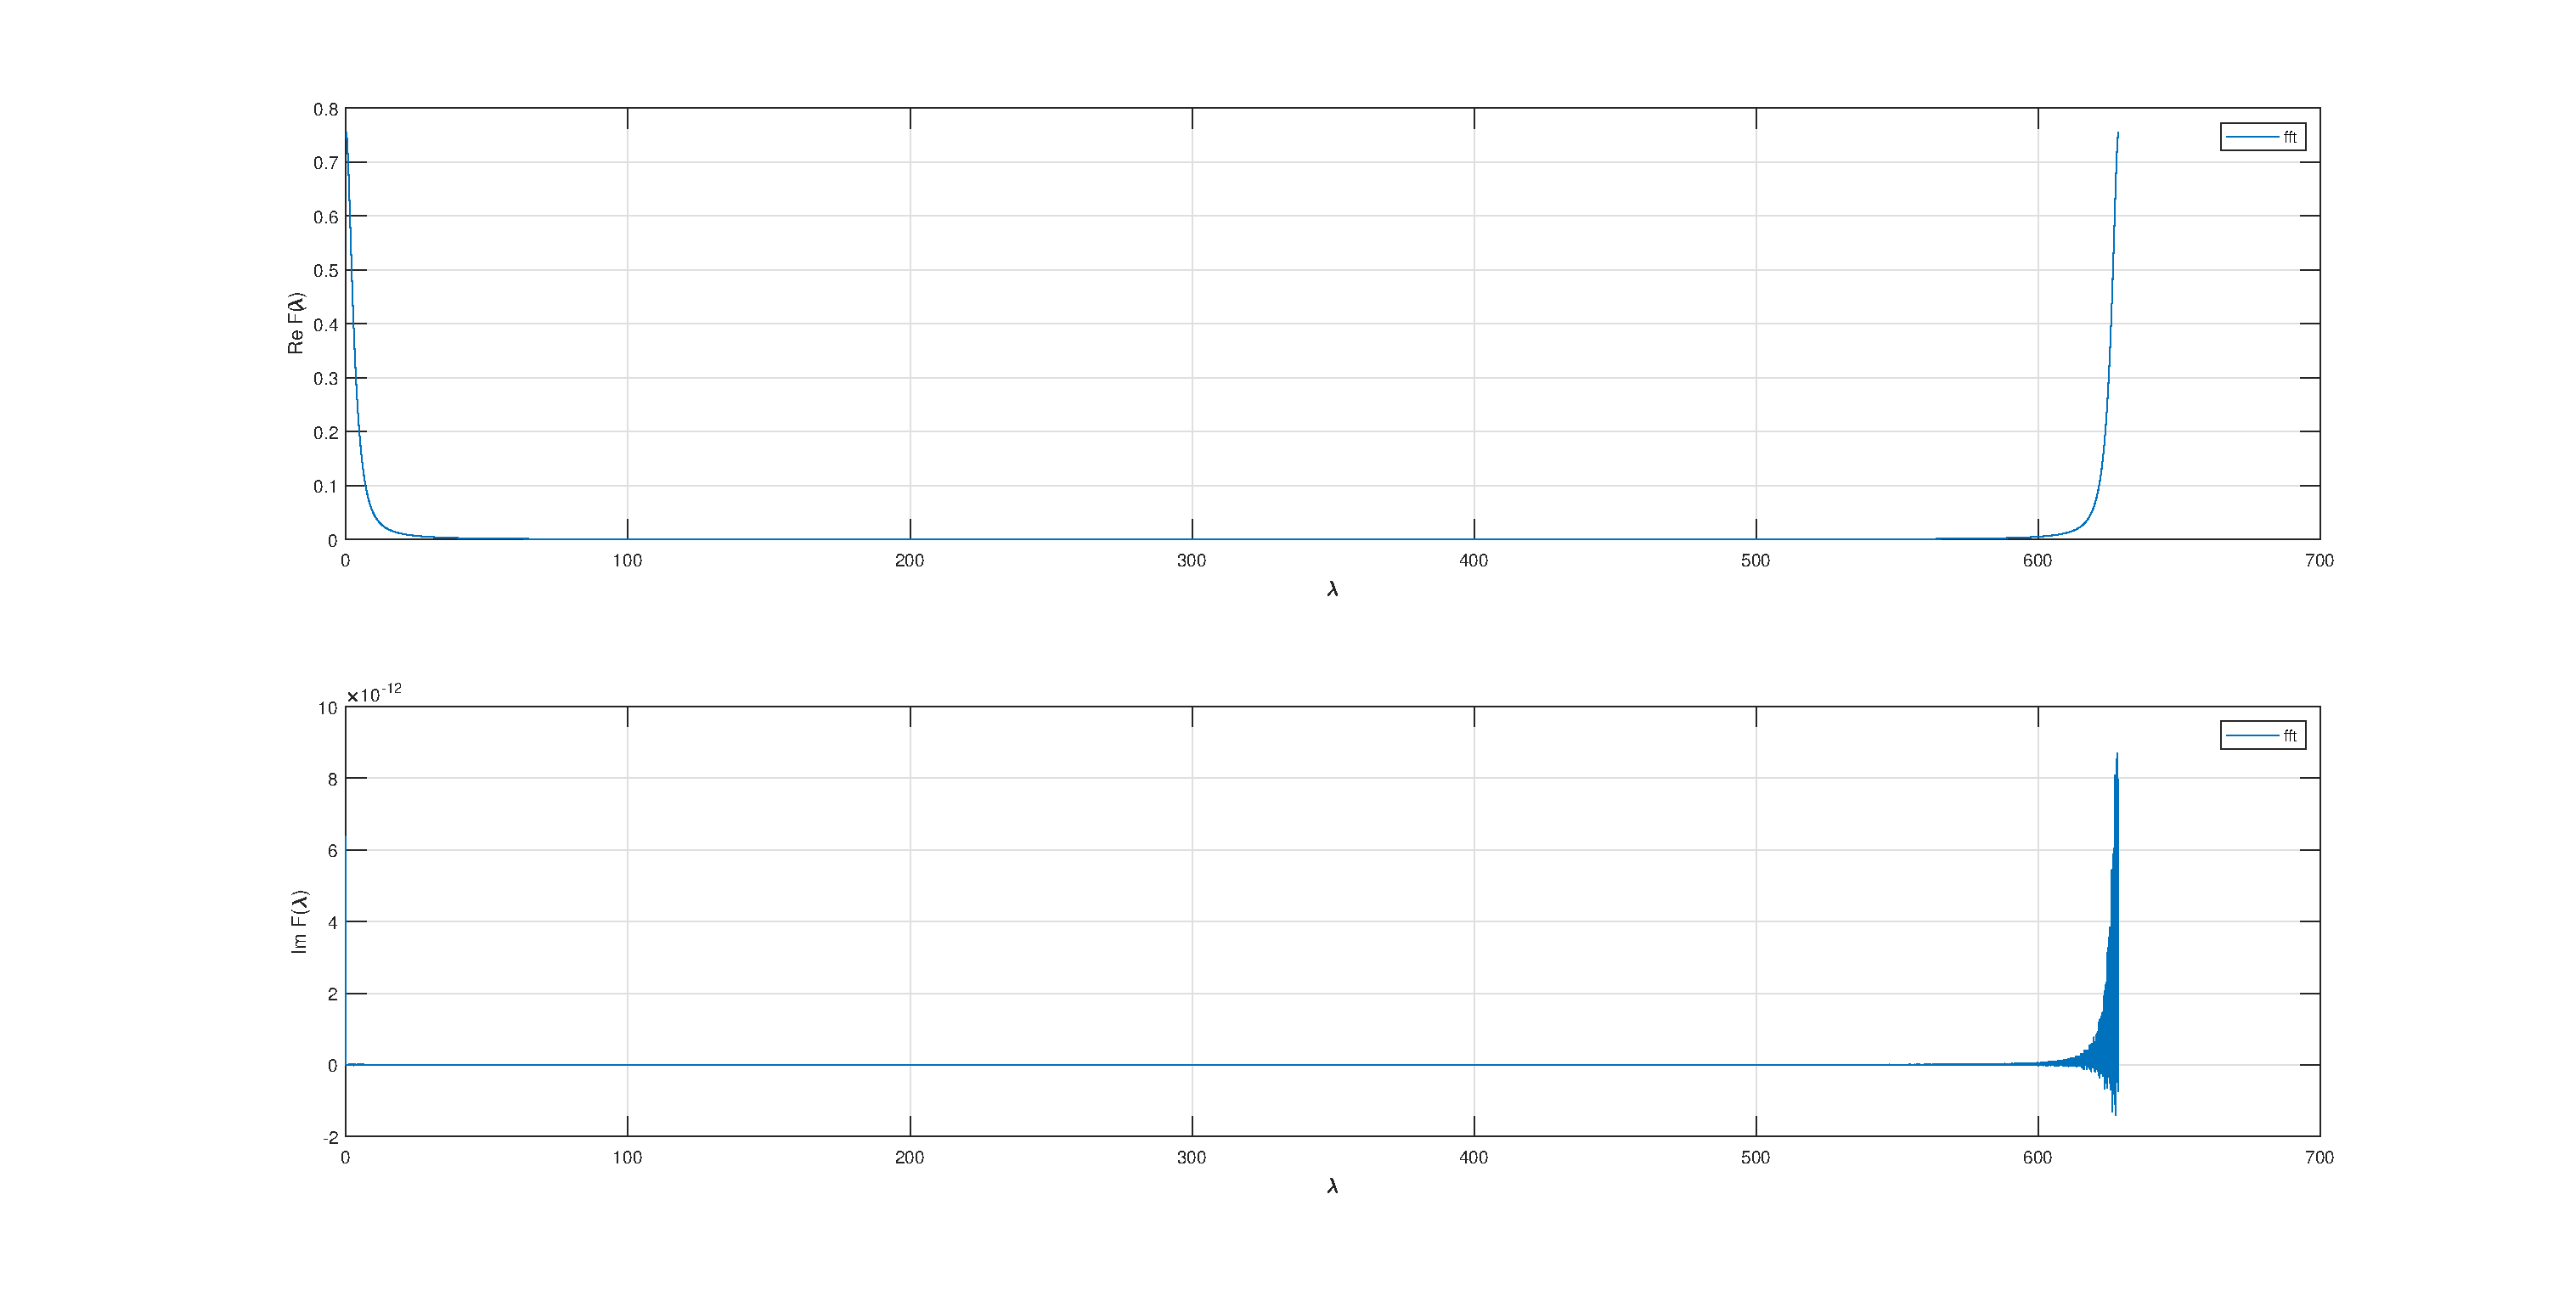
\includegraphics[width=1\textwidth]{f3.eps}
\newpage
\[f(t) = \frac{\sin(t^3)}{t^2}.\]
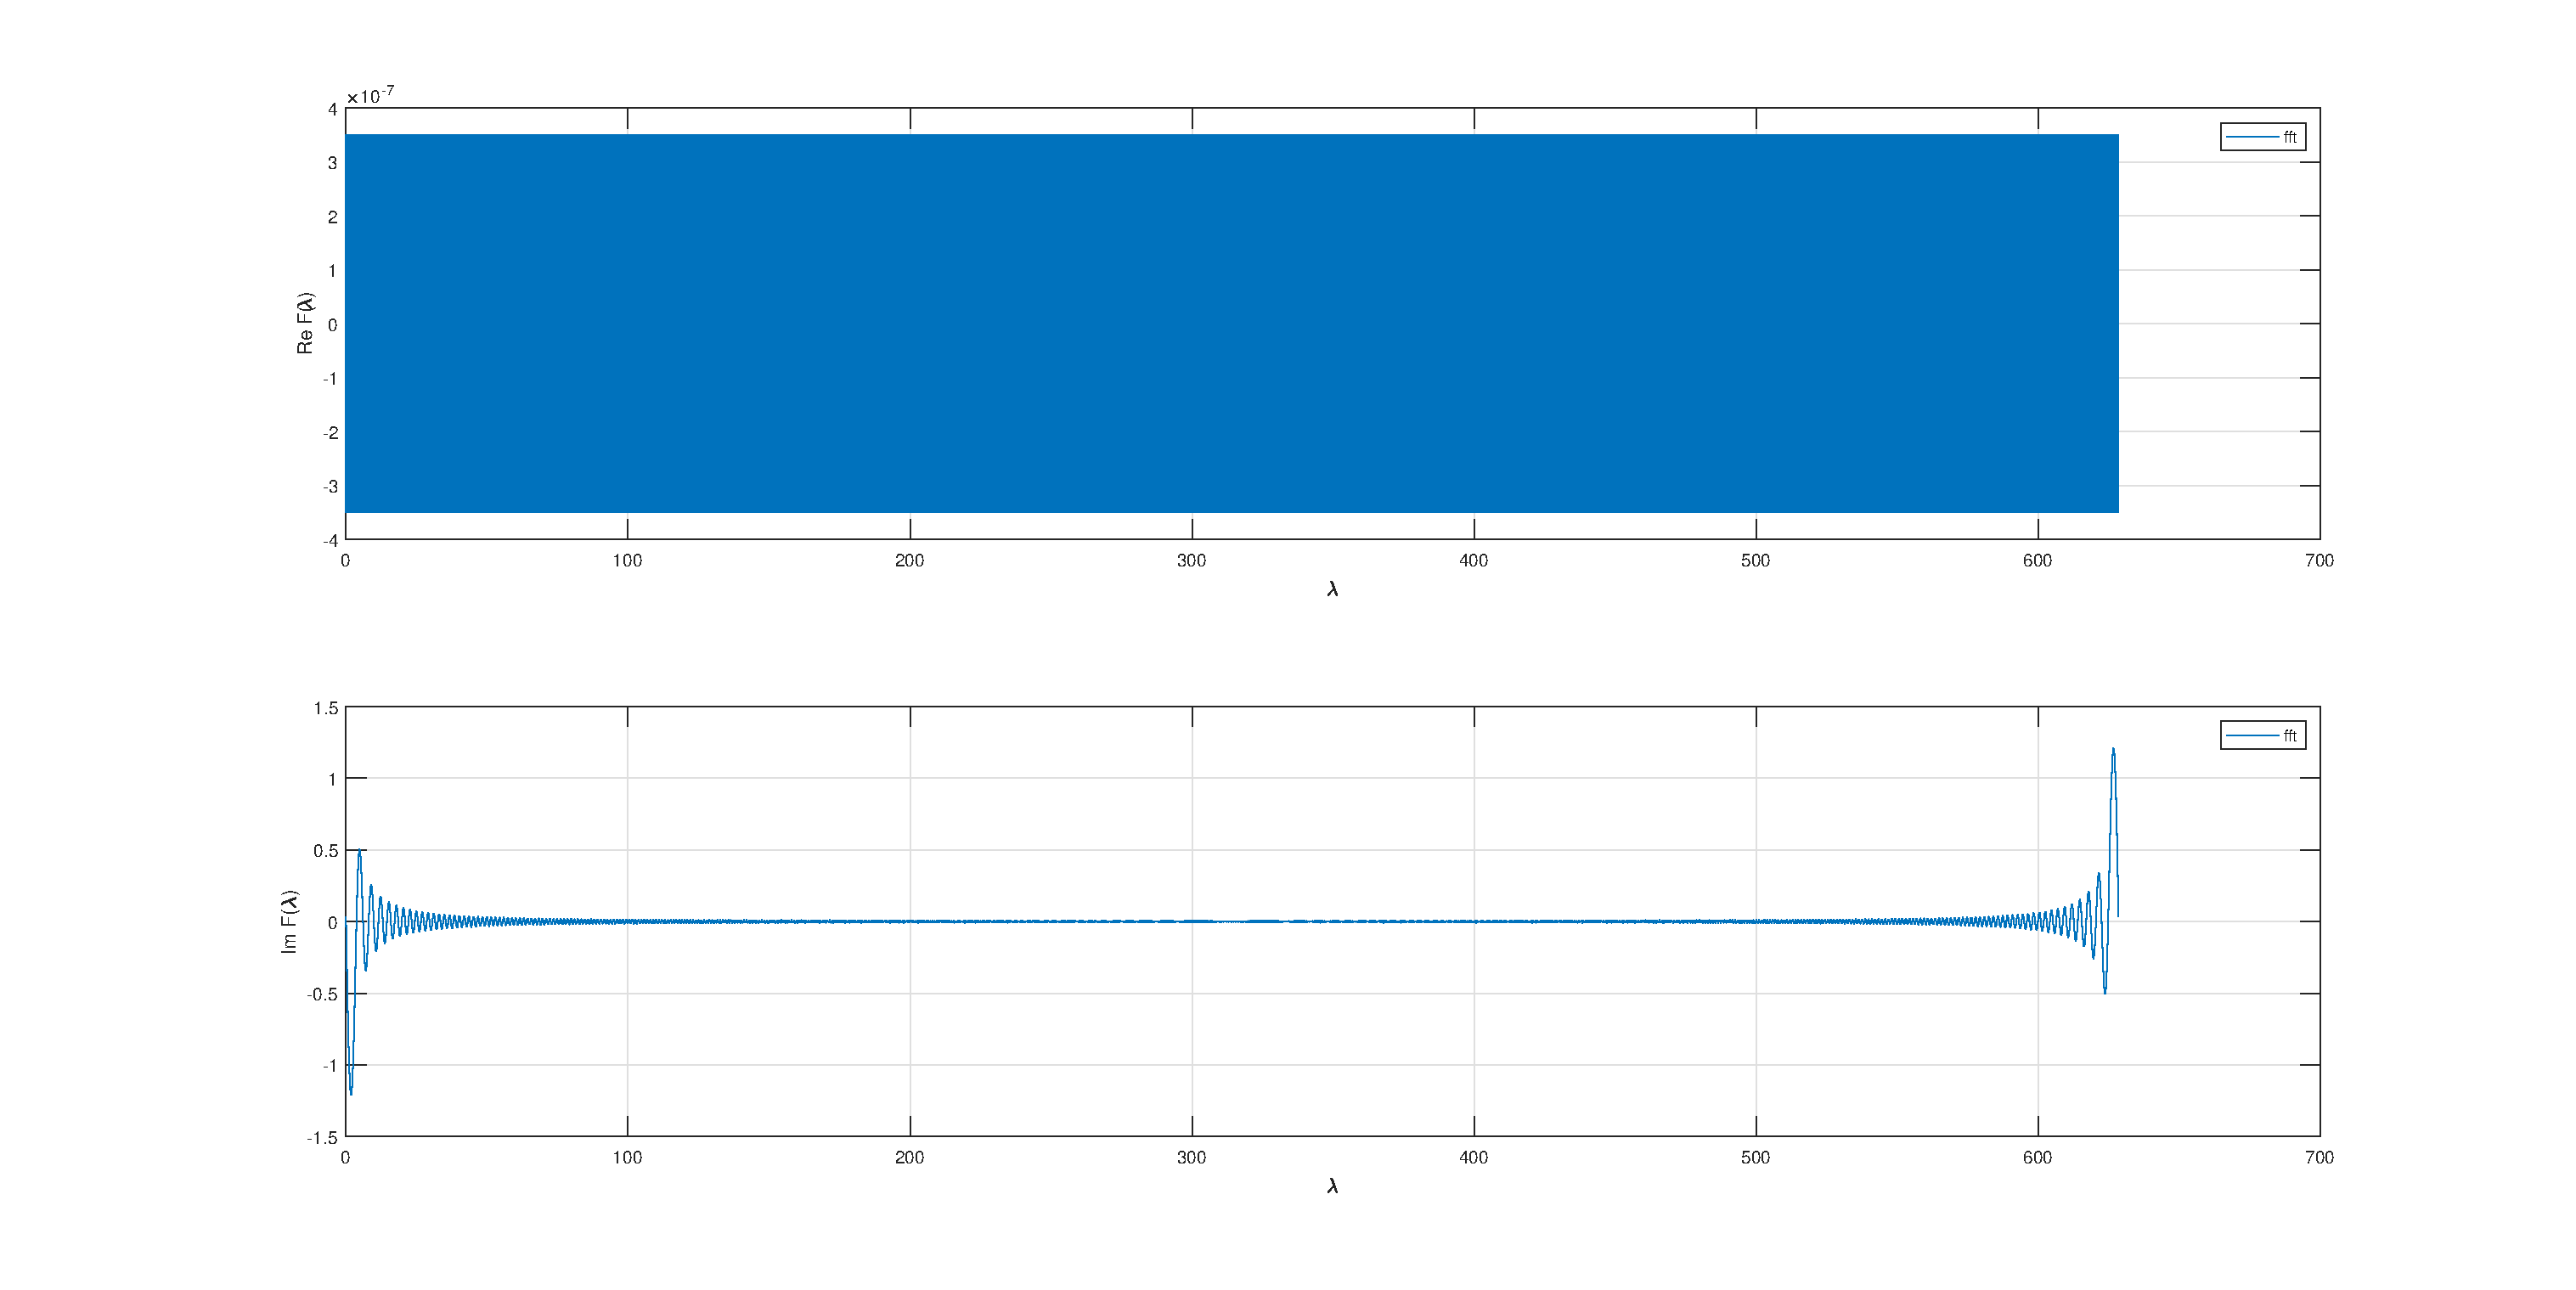
\includegraphics[width=1\textwidth]{f4.eps}

\section{Эффект наложения спектра и рябь}
После дискретизации сигнал переходит в размноженный спектр. Эффект наложения спектра проявляется, когда интервал спектра больше, чем расстояние между получившимися размноженными спектрами (если считать, что спектр ограничен). Рассмотрим для примера гауссиану $f(t) = e^\frac{t^2}{2}$, преобразованием которой является похожая функция $F(\lambda) = \sqrt{2 \pi} \cdot e^\frac{\lambda^2}{2}$. Ошибка наложения спектра будет возникать, когда $\frac{2 \pi}{\Delta t} < \Lambda$, где $\Lambda$ - интервал спектра. Можно считать, что спектр гауссианы ограничен и его интервал равен $2 \pi$ (для удобства). Тогда если взять шаг дискретизации $\Delta t = 2$, мы увидим эффект наложения спектра, в сравнении с несуммированным размноженным спектром:
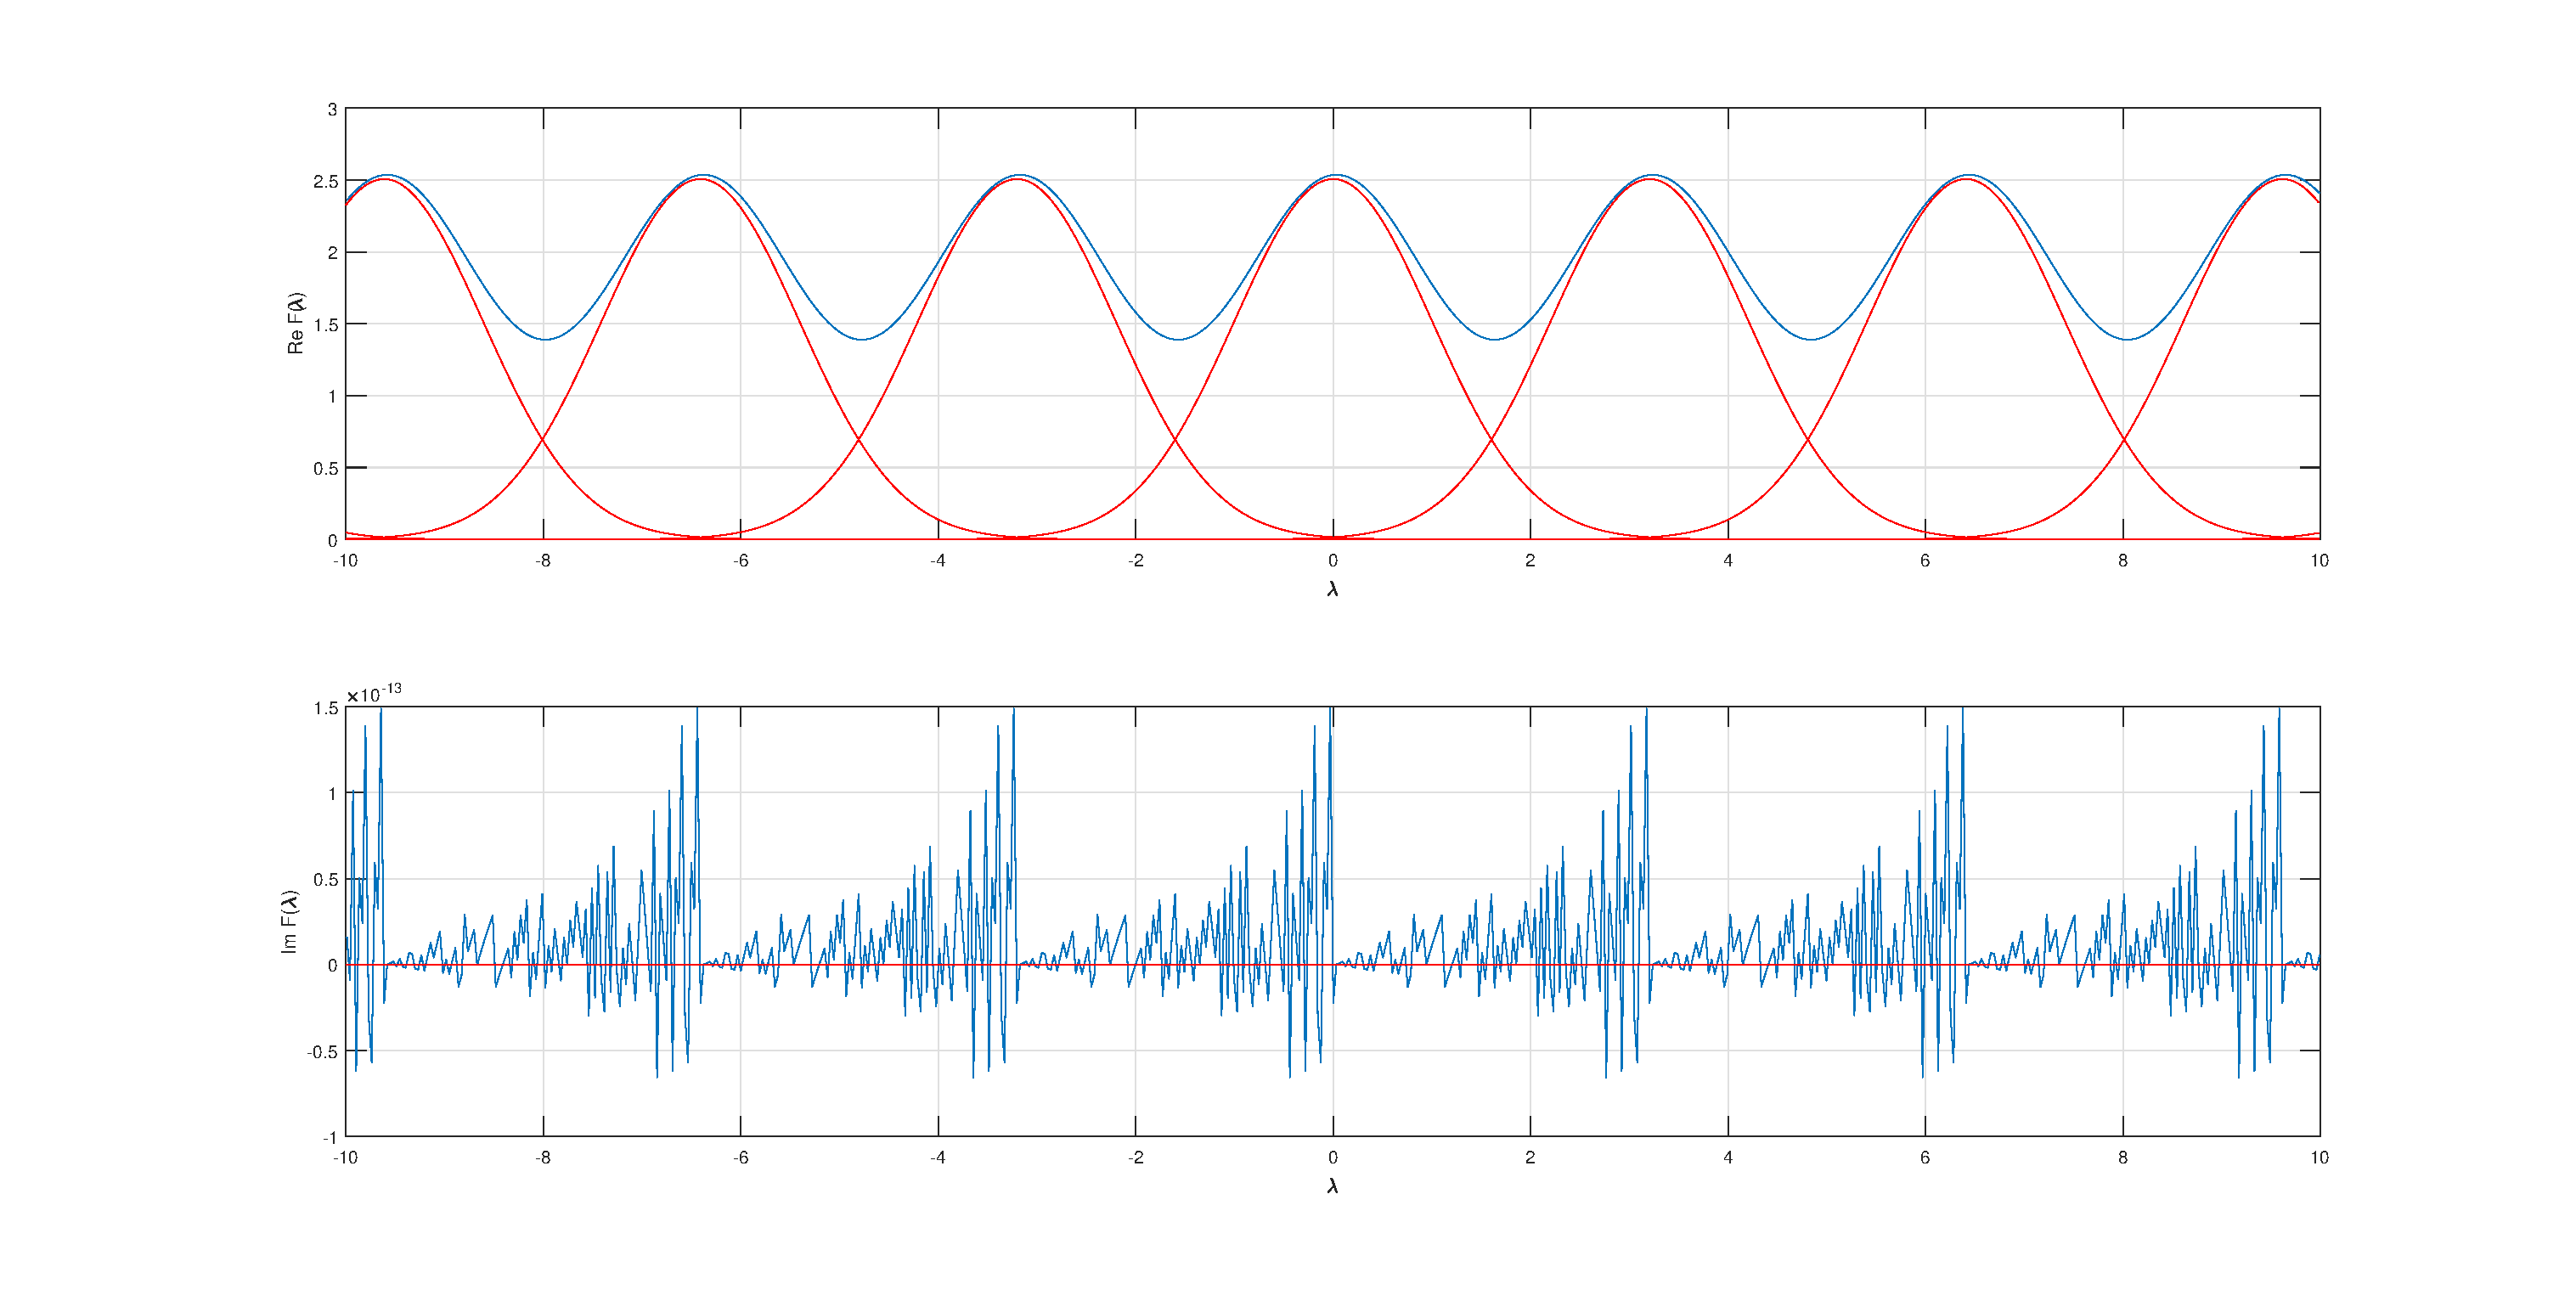
\includegraphics[width=1\textwidth]{aliasing1.eps}
Выбрав шаг $\Delta t = 1$, мы как раз попадаем ровно в интервал спектра, и эффект наложения спектра пропадает (на самом деле почти, потому что спектр гауссианы все же неограничен, но очень близок к нулю вне данного интервала). Такая частота называется частотой дискретизации Найквиста. (то есть $\Delta t  = \frac{2 \pi}{\Lambda}$)
\newline
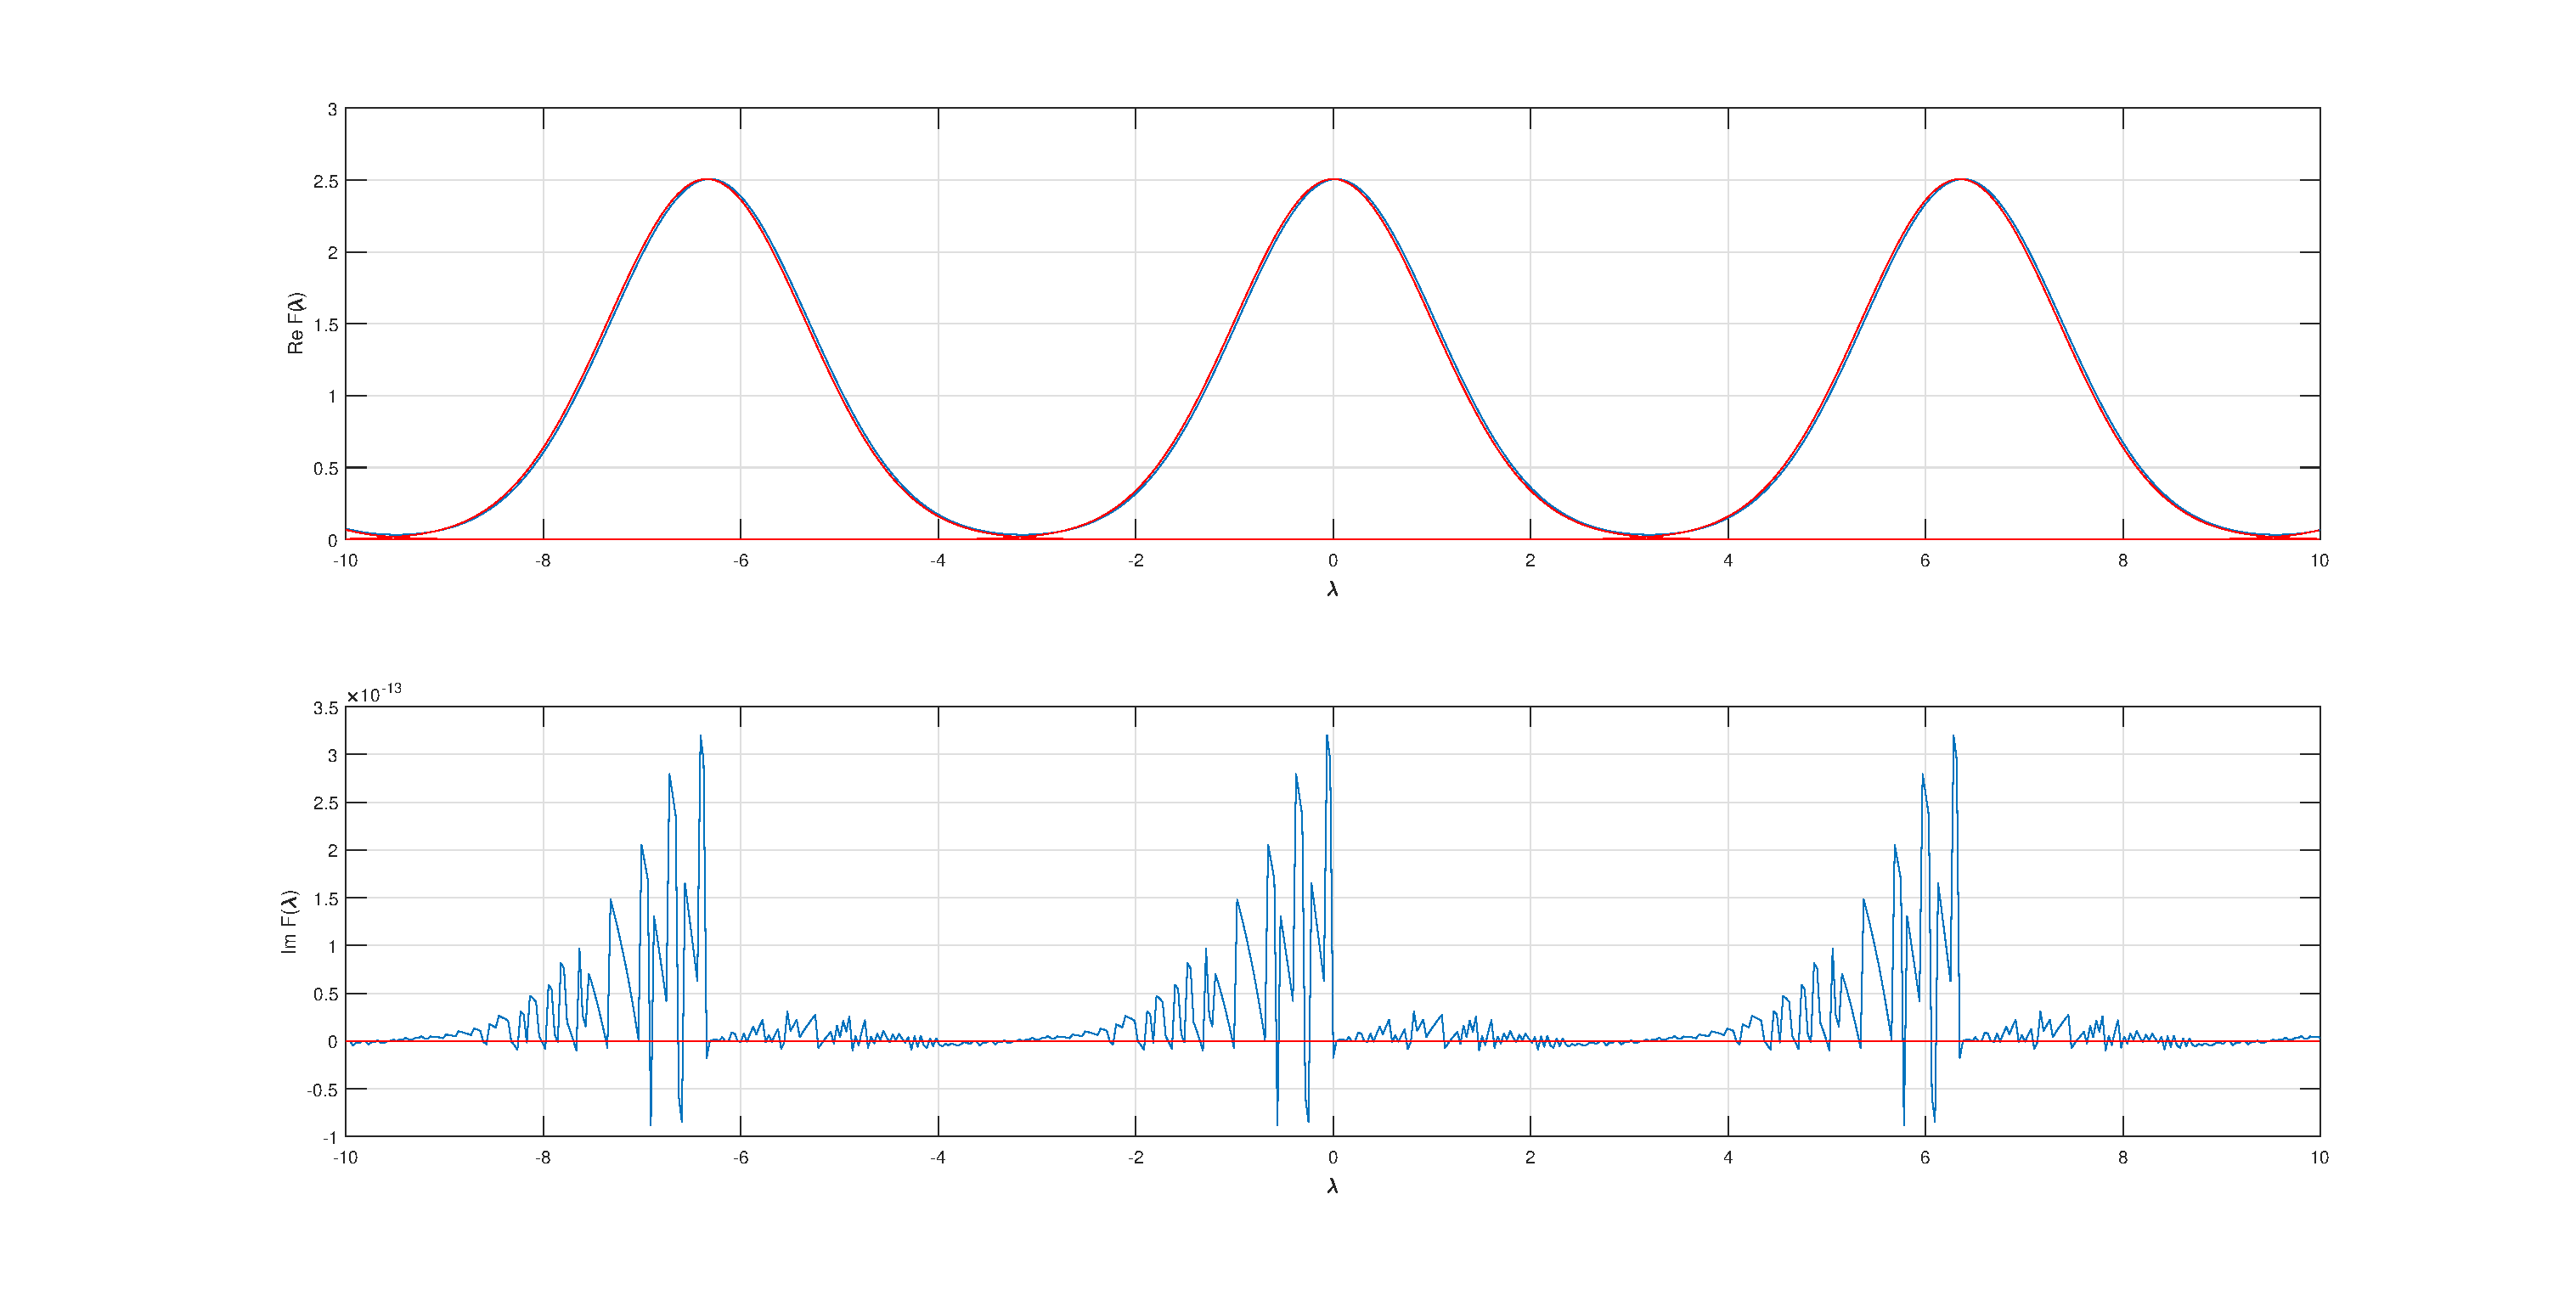
\includegraphics[width=1\textwidth]{aliasing2.eps}
Другим побочным эффектом ДПФ является рябь. Она связана с тем, что мы берем конечный промежуток для сигнала, в связи с тем теряем в точности. Особенно сильно этот эффект проявляется в точках разрыва спектра, как видно на примере функции номер 1:
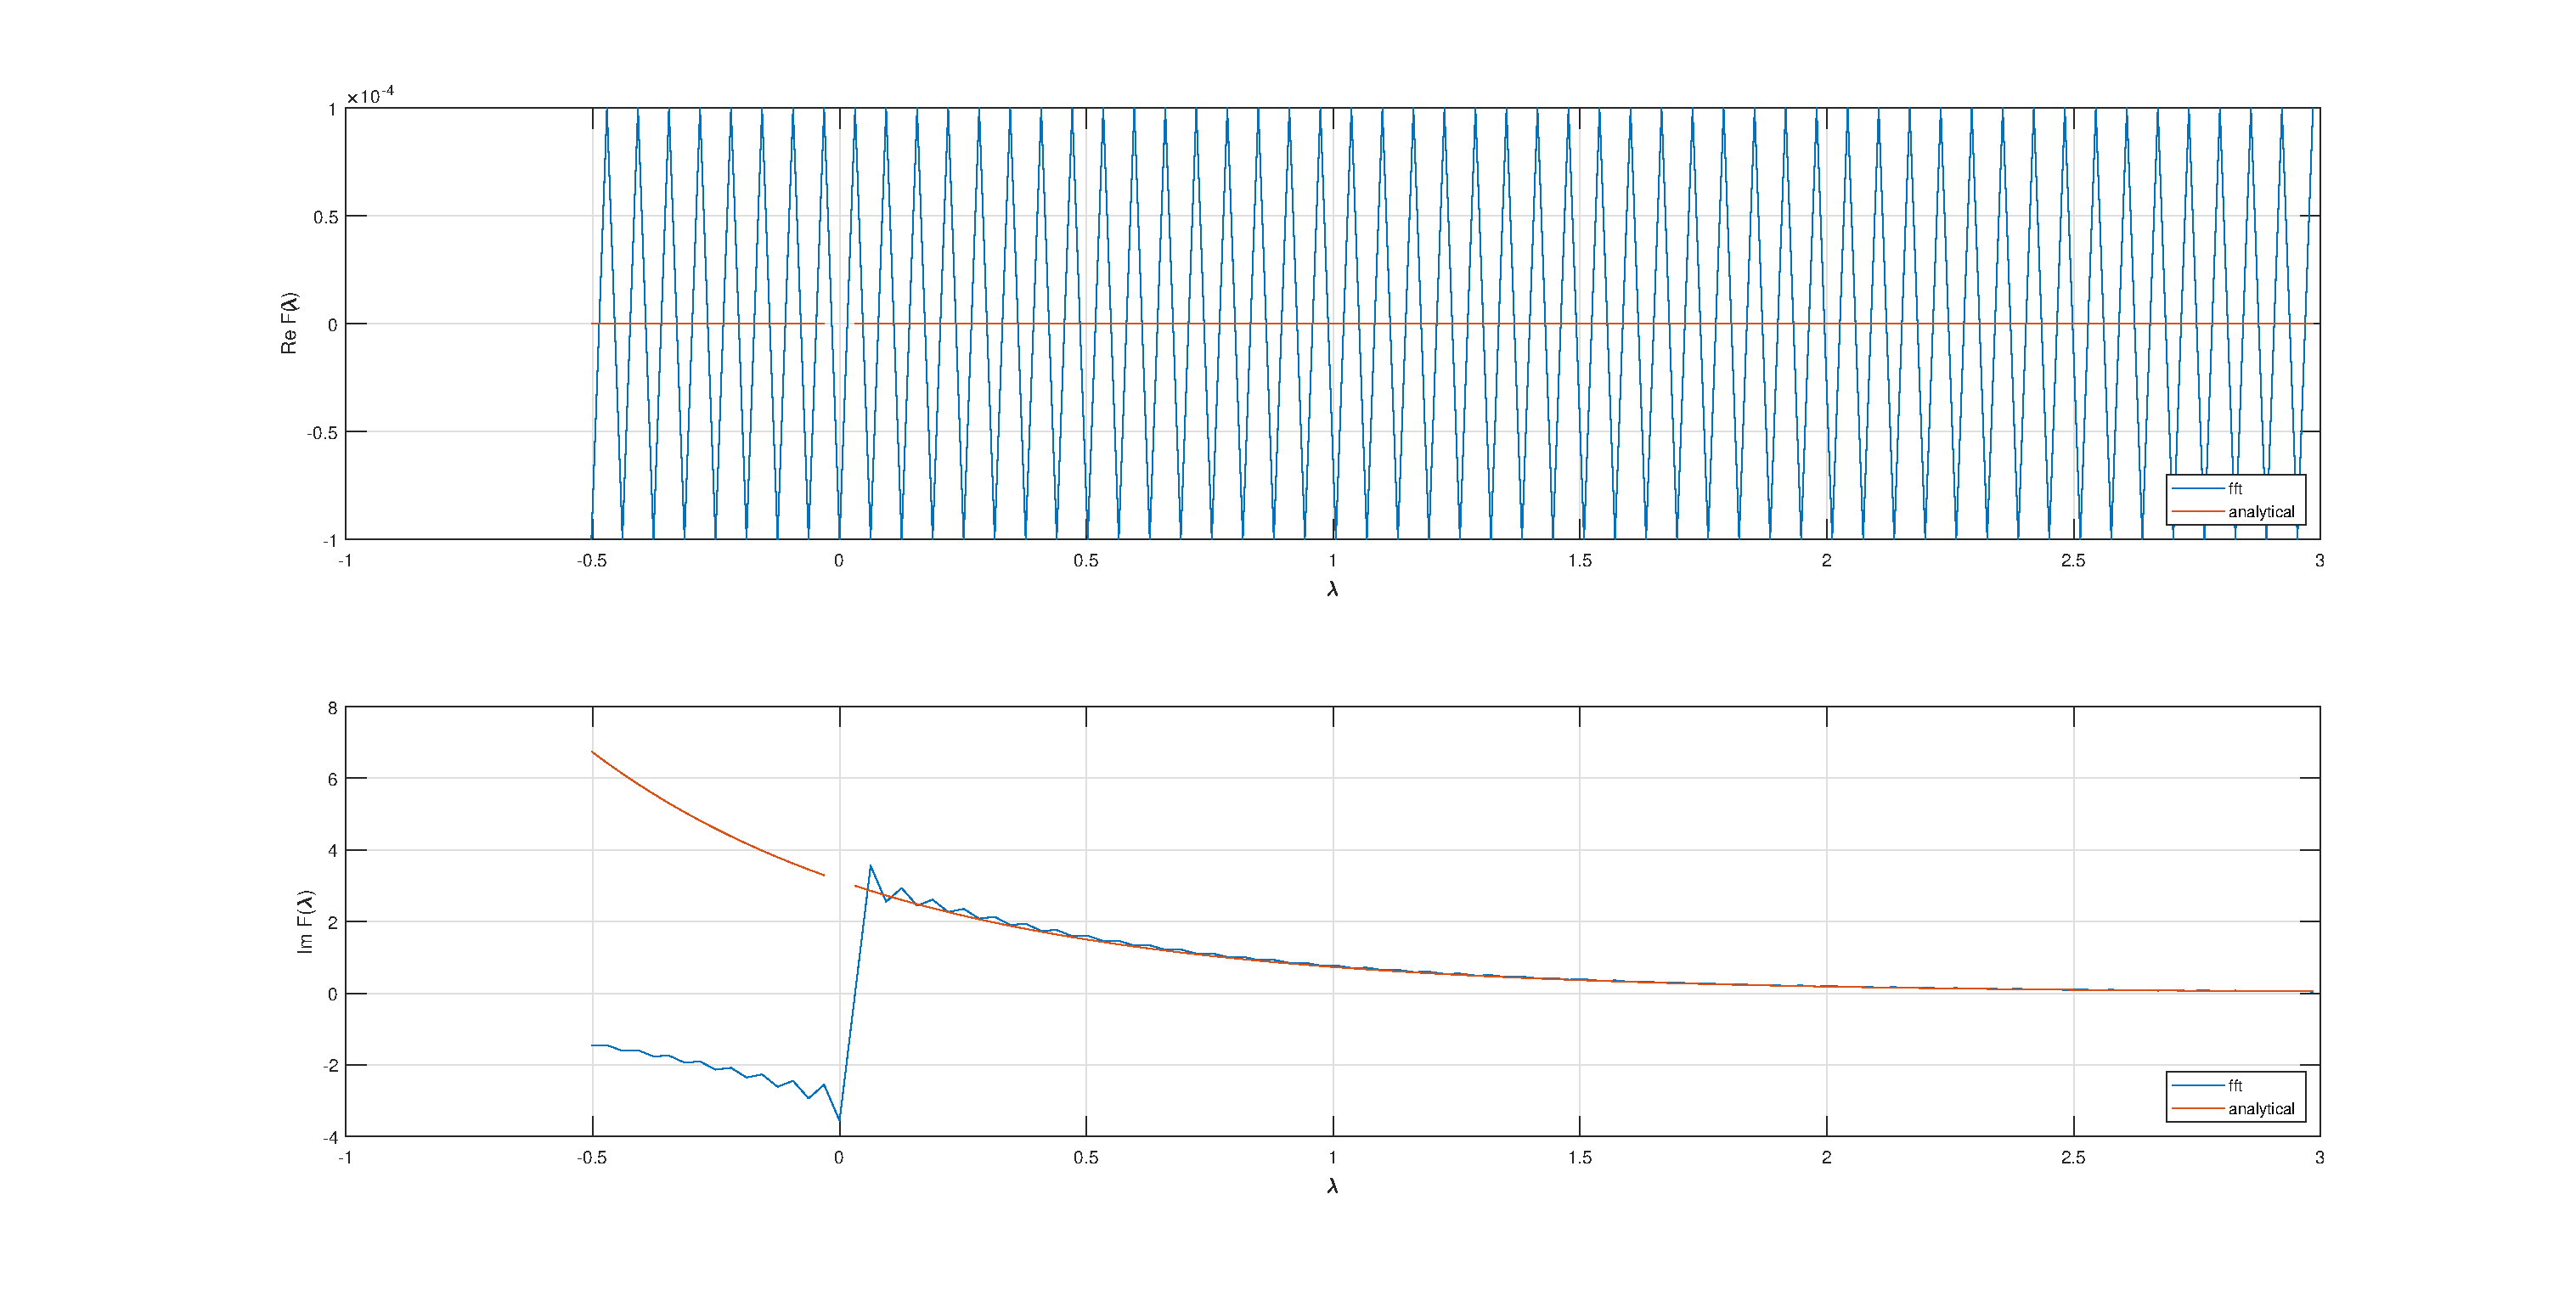
\includegraphics[width=1\textwidth]{f1.eps}
Увеличив интервал сигнала с [-100, 100] до [-1000, 1000], мы видим уменьшение эффекта ряби, хотя в точке разрыва до конца убрать его невозможно:
\newline
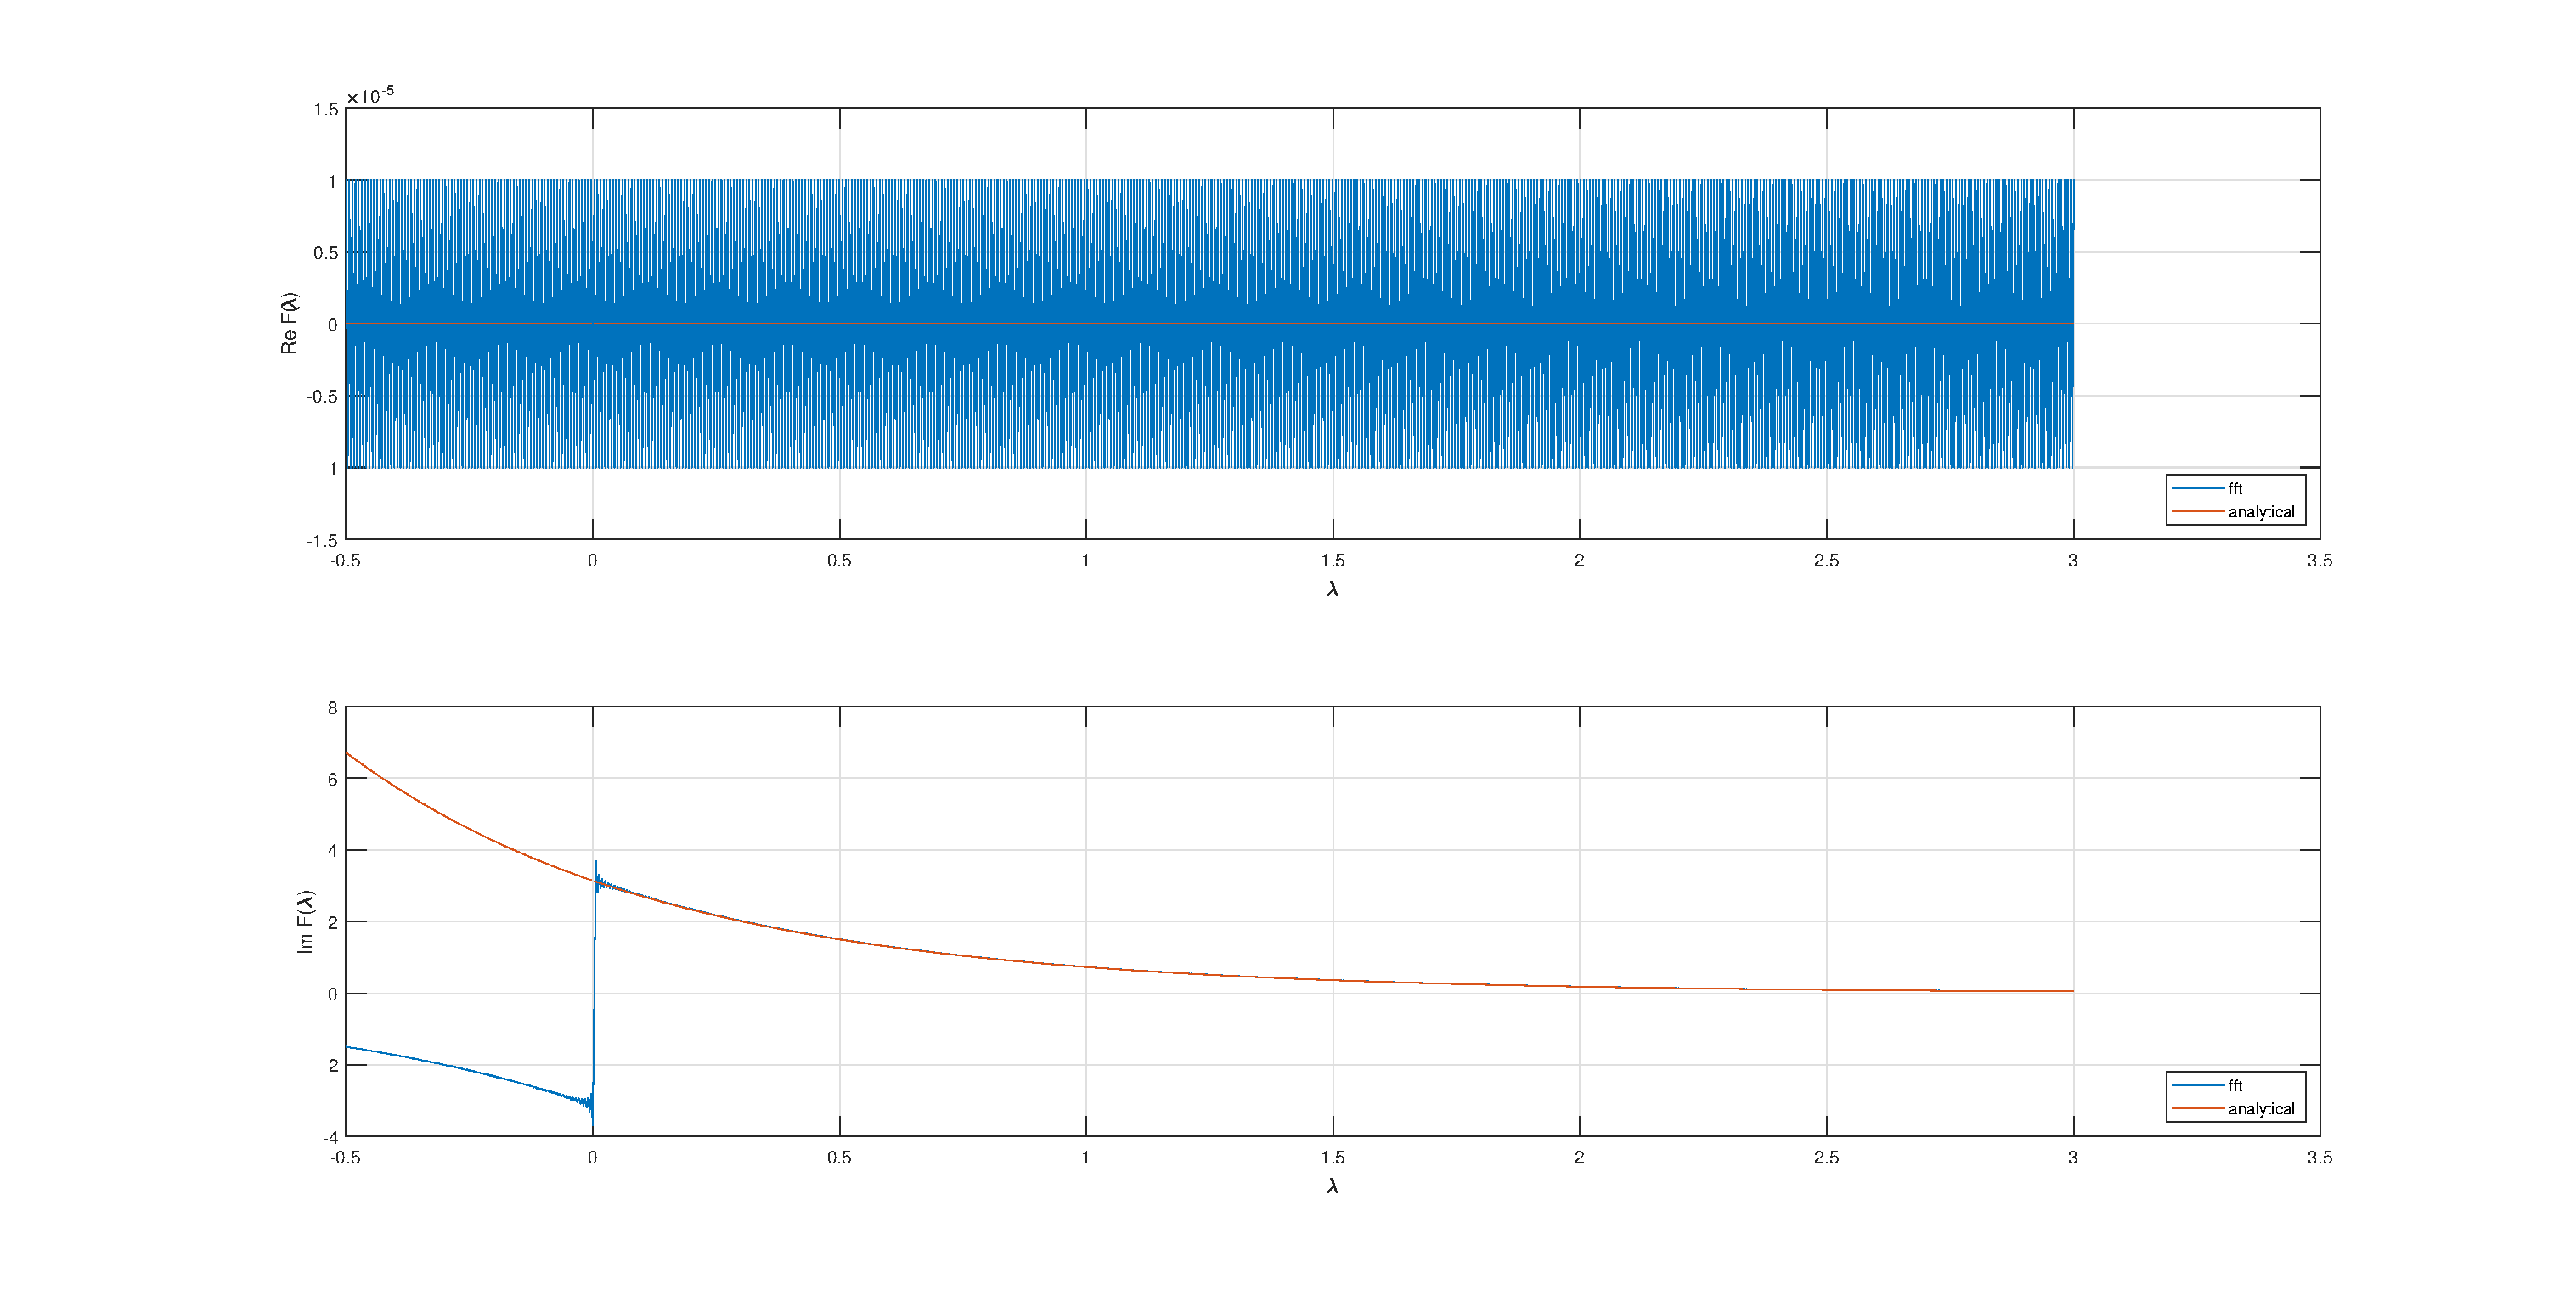
\includegraphics[width=1\textwidth]{f1_1.eps}
\begin{thebibliography}{99}
\bibitem{1} Точилин П.А. Лекции по Преобразованиям Лапласа Фурье 2024
\end{thebibliography}

\end{document}


